\section{Analyse der Tranceiver-Platinen}
Zu Verfügung steht eine Tranceiver-Platine. Ein Tranceiver ist eine Platine, die sowohl als Sender (Transmitter) als auch als Empfänger (Receiver) fungieren kann. Dafür ist diese Platine mit einem Transceiver-Chip ausgestattet, der Funktion teilweise abgeschaltet werden kann, sodass die Platine zu einem reinen Transmitter oder zu einem reinen Receiver wird.  
Hierfür stehen zwei Jumper zur Verfügung, die auf der Tranceiver-Platine platziert sind. Diese Jumper können gesteckt oder abgezogen werden, um die Funktionalität der Platine zu ändern. Hierbei ist der Platinenbeschriftung zu entnehmen, dass der TX (Transmitter) nur dann funktioniert, wenn man sowohl J1 und J2 ausgesteckt hat (eine Eingangsspannung liegt dann an dem Transceiver-Chip auf beiden Teilmodulen an)

Die Jumpers sind auf der Abbildung \ref{fig:Tranceiver-Platine} zu sehen.
\begin{figure}[H]
    \centering
    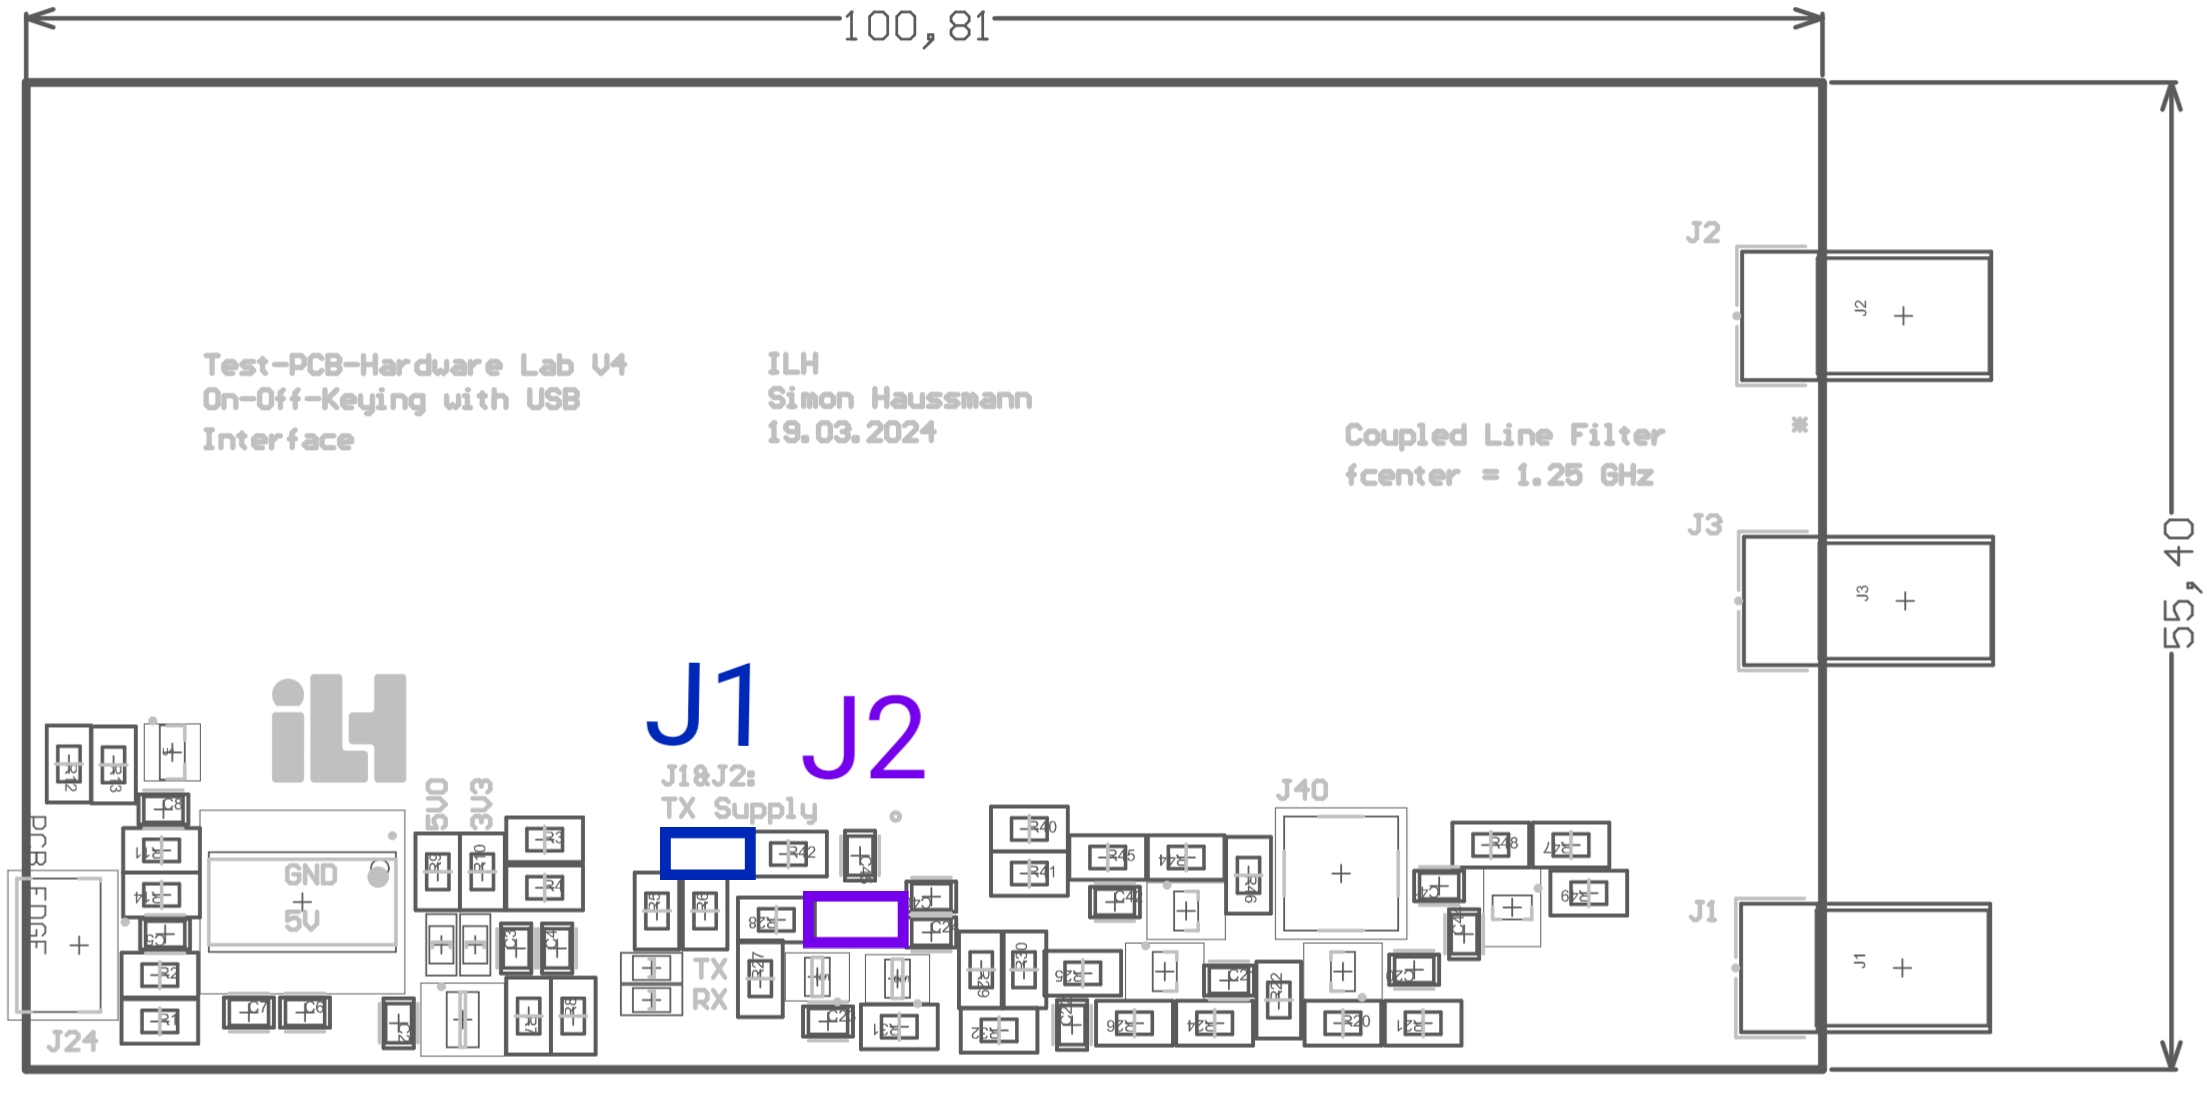
\includegraphics[width=0.8\textwidth]{Pictures/Jumper.jpg}
    \caption{Tranceiver-Platine mit Jumpern J1 und J2. Quelle: vgl. Litertaturverzeichnis \cite{SchaltplanPCBV4}: Schaltpläne der Platine V4}
    \label{fig:Tranceiver-Platine}
\end{figure}
\subsection{Funktion der Jumper auf der Tranceiver-Platine}
\subsubsection{J1}
Der J1 hat die Funktion, den Trasmitter abzuschalten. Wenn der Jumper J1 gesteckt ist, wird der Modul des Transmitters überbrückt.
\subsubsection{J2}
Der J2 hat die Funktion, den Receiver abzuschalten. Wenn der Jumper J2 gesteckt ist, wird der Modul des Receivers überbrückt. 

Es ist auch wichtig zu beachten, dass ohne den Receiver der Transmitter nicht funktionieren kann. Das bedeutet, dass der Jumper J2 immer abgezogen sein muss, damit der Transmitter funktioniert. Dies ist auf die eingeschaften des zur Verfügung stehenden Transceiver-Chips zurückzuführen.

\subsection{Serielles Protokoll UART}
Universal Asynchronous Receiver/Transmitter (UART) stellt ein serielles Protokoll dar, also einen Regelsatz für den Austausch von Daten zwischen zwei Geräten. Das Protokoll ist asynchron, was bedeutet, dass es kein gemeinsamer Taktsignal zwischen dem Sender und dem Empfänger gibt. Stattdessen müssen beide Seite auf dieselbe Bit- und Baudrate eingestellt
Zudem müssen die beiden Seiten dieselbe Rahmenstruktur und dieselben Parameter nutzen. Das UART-Protokoll ist simpel und ermöglicht die Signalübertragung in beide Richtungen über lediglich zwei Drähte zwischen Sender und Empfänger. Das Signal wird in einem vom Protokoll bestimmten Format gesendet.\footnote{Vgl. Rohde \& Schwarz: UART verstehen. Online: \url{https://www.rohde-schwarz.com/de/produkte/messtechnik/essentials-test-equipment/digital-oscilloscopes/uart-verstehen_254524.html} (abgerufen am 07.07.2025).} 

Die Kommunikation über UART kann in verschiedenen Formaten, nämlich im:
\begin{itemize}
    \item Simplex-Betrieb
    \item Halbduplex-Betrieb
    \item Voll-Duplex-Betrieb
\end{itemize}
erfolgen.

Das Rahmenformat von UART sieht folgendermaßen aus:
\begin{figure}[H]
    \centering
    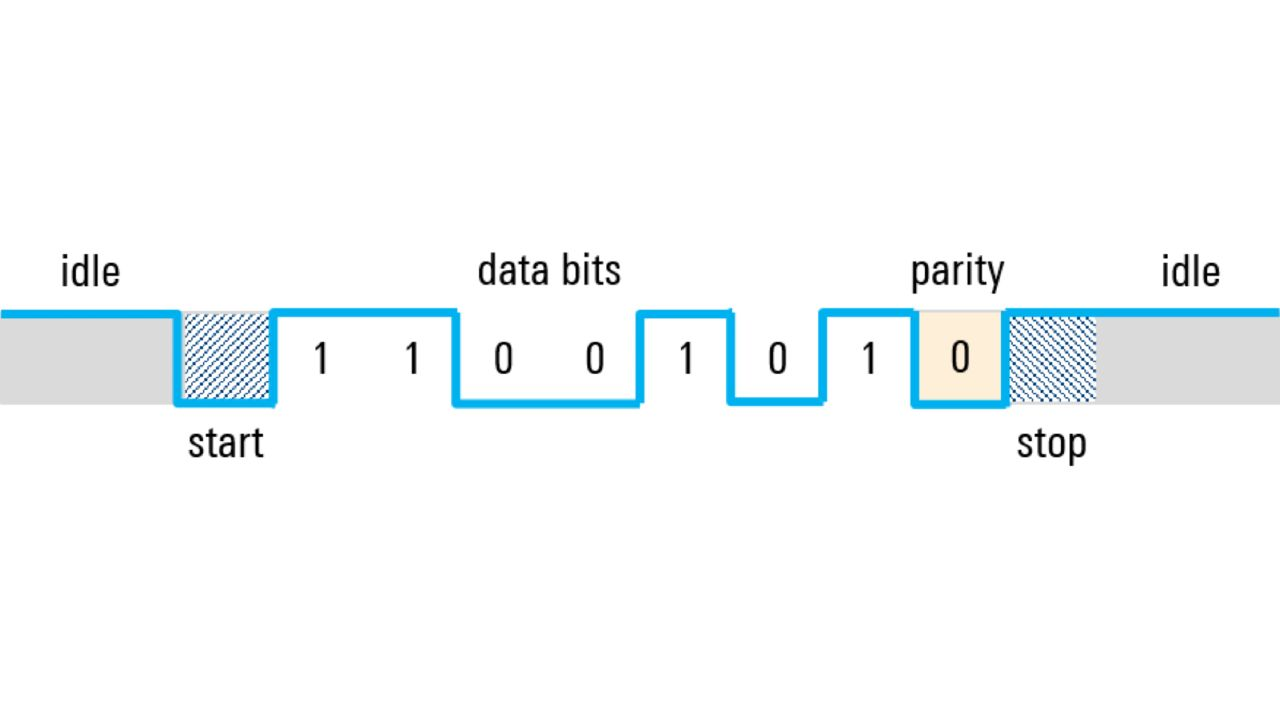
\includegraphics[width=0.8\textwidth]{Pictures/UART-Frame.jpg}
    \caption{Rahmenformat von UART. Quelle: \url{https://cdn.rohde-schwarz.com/image/products/test-and-measurement/essentials-test-equipment/essentials-digital-oscilloscopes/understanding-uart-02-infographic-rohde-schwarz_200_112521_1024_576_7.jpg}}
    \label{fig:UART-Frame}
\end{figure}

Die Übertragung erfolgt in Form von Bytes, die aus 8 Datenbits bestehen. UART-Rahmen enthalten Start- und Stoppbits und Datenbits, die die tatsächliche Information tragen. Wie bei den meisten digitalen Systemen ist es vom UART-Protokoll festgelegt, dass der HIGH-Pegel einer logischen "1" und der LOW-Pegel einer logischen "0" entspricht. Eine spezifische Spannungsschwelle ist aus Flexibilitätsgründen durch UART nicht festgelegt, weswegen der HIGH-Pegel als "Mark" und der LOW-Pegel als "Space" beschrieben wird. Doch es ist zu beachten, dass das System beim UART-Protokoll im Ruhezustand (engl. idle) bei einem HIGH-Pegel liegt. Dies hat den Sinn, dass man bei einer beschädigten Leitung durch einen konstanten LOW-Pegel im Ruhezustand eine defekte Leitung/Verbindung bzw. einen defekten Sender erkennen kann.\footnote{Vgl. Rohde \& Schwarz: UART verstehen. Online: \url{https://www.rohde-schwarz.com/de/produkte/messtechnik/essentials-test-equipment/digital-oscilloscopes/uart-verstehen_254524.html} (abgerufen am 07.07.2025).}

Der Startbit signalisiert den Beginn der Datenübertragung. Hierbei übergeht der Sender aus dem Ruhezustand (HIGH-Pegel) in den LOW-Pegel, um dem Empfänger zu signalisieren, dass die Datenübertragung beginnt. 
Unmittelbar danach folgen die Datenbits, die das Nutzsignal übertragen. Die Datenbits werden nacheinander gesendet, wobei eine Übertragung von 5 bis 9 Bits pro Byte erlaubt ist, jedoch eine Übertragung von 7 oder 8 Bits pro Byte am häufigsten verwendet wird. Die Reihenfolge der Datenbits wird dabei vom Sender invertiert und mit dem Least Significant Bit (LSB) zuerst gesendet. Das Most Significant Bit (MSB) wird zuletzt gesendet.
Nach einer erfolgreichen Übertragung der Nutzdaten übergeht der Sender zurück in den Ruhezustand (HIGH-Pegel), um dem Empfänger zu signalisieren, dass die Übertragung abgeschlossen ist.
In einigen Fällen kann es auch vorkommen, dass ein zweites (optionales) Stoppbit konfiguriert wird, um dem Empfänger Zeit für den nächsten Übertragungsrahmen zu gewähren. Dies wird jedoch in der Praxis selten umgesetzt.\footnote{Vgl. Rohde \& Schwarz: UART verstehen. Online: \url{https://www.rohde-schwarz.com/de/produkte/messtechnik/essentials-test-equipment/digital-oscilloscopes/uart-verstehen_254524.html} (abgerufen am 07.07.2025).}

Zuletzt sollte man noch erwähnen, dass manchmal ein Paritätsbit zur Verwendung kommt. Dieser trägt zur Fehlererkennung bei, indem es die Anzahl der gesetzten Bits (1-Bits) in einem Byte überprüft. Es gibt zwei Arten von Paritätsbits: 
\begin{itemize}
    \item Gerade Parität: Hier wird das Paritätsbit so gesetzt, dass die Gesamtanzahl der 1-Bits im Byte gerade ist.
    \item Ungerade Parität: Hier wird das Paritätsbit so gesetzt, dass die Gesamtanzahl der 1-Bits im Byte ungerade ist.
\end{itemize}

Das Paritätsbit kann jedoch nur ein einziges gekipptes (also falsch übertragenes) Bit erkennen, aber nicht korrigieren. Es kann auch nicht erkennen, ob zwei oder mehr Bits gekippt wurden. Daher ist es in der Praxis nicht sehr verbreitet und wird oft weggelassen.\footnote{Vgl. ebenda}

Bei unserer tatsächlichen Schaltung liegt auch ein Standard-UART-Protokoll vor, das eine Baudrate von 115200 Baud und eine Datenübertragung von 8 Datenbits, 1 Stoppbit und ohne Paritätsbit verwendet. Man erkennt auch den Ruhezustand daran, dass bei einem fehlenden Sendesignal die an der Schaltung Diode für "TX" leuchtet, also den HIGH-Pegel anzeigt.

\section{Pegelplanrechnung}
\subsection{Rekapitulation des Link-Budgets}
\subsection{Rekapitulation der Sensitivität}
\subsection{Berechnung des Pegelplans}